\section{Spacecraft Control Architecture Rapid Simulator (SCARS) Toolbox}\label{sec:toolbox}
    This chapter consists of description of the toolbox designed as a part of this thesis work. After the following introduction, in Sections \ref{toolbox:objectives}, \ref{toolbox:software} and \ref{toolbox:architecture} the objectives of the toolbox and its high level structures are described. After that, one finds theoretical description of satellite mechanics and coordinated systems, with following descriptions of theoretical principles of each major component of the toolbox and their implementation in MATLAB and Simulink software. At the end, methods of visualization of acquired simulations are discussed.  

    To fullfil the main objective of this thesis, that is to provide the community of beginner control engineers with a satellite control system prototyping toolbox, a self-made solution is proposed. This chapter provides the insight into the architecture of \ac*{scars} Toolbox, a software framework created for purposes of this thesis in MATLAB and Simulink. First the main objectives of that solution are stated, then architecture of \ac{scars} is described, to give the initial description of how the toolbox can be used. In following sections the principles of operation of each major part of the toolbox, and how they were implemented, are presented.

    The inputs of \ac{scars} Toolbox - whether used as a parts library and integrated into own project, or as ready-made modular simulation - are parameters of spacecraft hardware, such as for example size of the satellite, trusters operational range, and initial mission parameters, for example time, Keplerian elements or initial body rates. The outputs of the toolbox are performances of each part and simulated behavior of the whole spacecraft, allowing the user to easily test different designs for their satellites.

\subsection{Objectives}\label{toolbox:objectives}
    The toolbox itself covers first two objectives of the the thesis. Following listing further specifies what should be expected of the end product and what features the users should be able to find in \ac{scars} Toolbox: 
    \begin{itemize}
        \item A model of orbital dynamics of Earth orbiting satellite;
        \item Models of most common satellite actuators and sensors and parametrize them, so that the actual hardware can be reproduced in simulation using values from datasheets;
        \item Modelled sources of environmental forces and torques, including most sources most relevant for small satellites;
        \item Several most basic control methods;
        \item Simulink Custom Library, with all models masked for quick set up;
        \item Methods of conducting preliminary review of feasibility of used hardware components and control methods;
        \item Interfaces allowing the user to connect the toolbox with visualization software.
    \end{itemize}

\subsection{Choice of software}\label{toolbox:software}
    To fit with the objectives of accessibility and ease of modification MATLAB family of software was chosen. MATLAB is one of the most popular scripting language and with the addition of Simulink software it can become powerful tool with the ability to set up numerical simulations in short time. MATLAB is taught in most technical universities and there is significant number of both courses available online and materials for self-teaching. For one purpose (described in Section \ref{sec:ksp}) a Python script acting as a dataflow bridge was used, as it was a simplest method to solve a problem described in that chapter. Several other software solutions were used for visualization purposes, with the reasoning described in Section \ref{sec:visualization}.

    Versatility of MATLAB may be attributed to the number of Add-Ons available for it. \ac{scars} Toolbox uses and requires the following modules:
    \begin{itemize}
        \item Aerospace Toolbox
        \item Navigation Toolbox
        \item CubeSat Simulation Library
        \item Control System Toolbox
        \item Simulink 3D Animation
    \end{itemize}
    
    %todo: cite courses and tutorials

\subsection{Architecture}\label{toolbox:architecture}
    \ac{scars} is divided into two parts: 1) Parts Library and 2) Modular Simulation. The Parts Library contains Simulink subsystems, which can be connected to form simulations of various complexity and for multiple scenarios. The other is a Modular Simulation, which can be set up with either MATLAB command line scripts or graphical user interface.

    \subsubsection{Parts Library}
        %TODO: Should I write something about the aim of the library?
        \ac{scars} Parts Library is a ready to use Simulink Custom Library, that is a collection of blocks available to use in Simulink models. All blocks in library downloaded alongside \ac{scars} are parametrized, masked and described to ease the integration of library parts into user simulation. The library is divided into specific sections: Satellite Models, Control Algorithms, Actuators, Sensors, Environment, Visualization, Example scenarios and Other blocks.
        % \begin{itemize}
        %     \item Satellite Models
        %     \item Control Algorithms
        %     \item Actuators
        %     \item Sensors
        %     \item Environment
        %     \item Visualization
        %     \item Example scenarios
        %     \item Other blocks 
        % \end{itemize}
% 
        \begin{figure}[H]
            \centering
            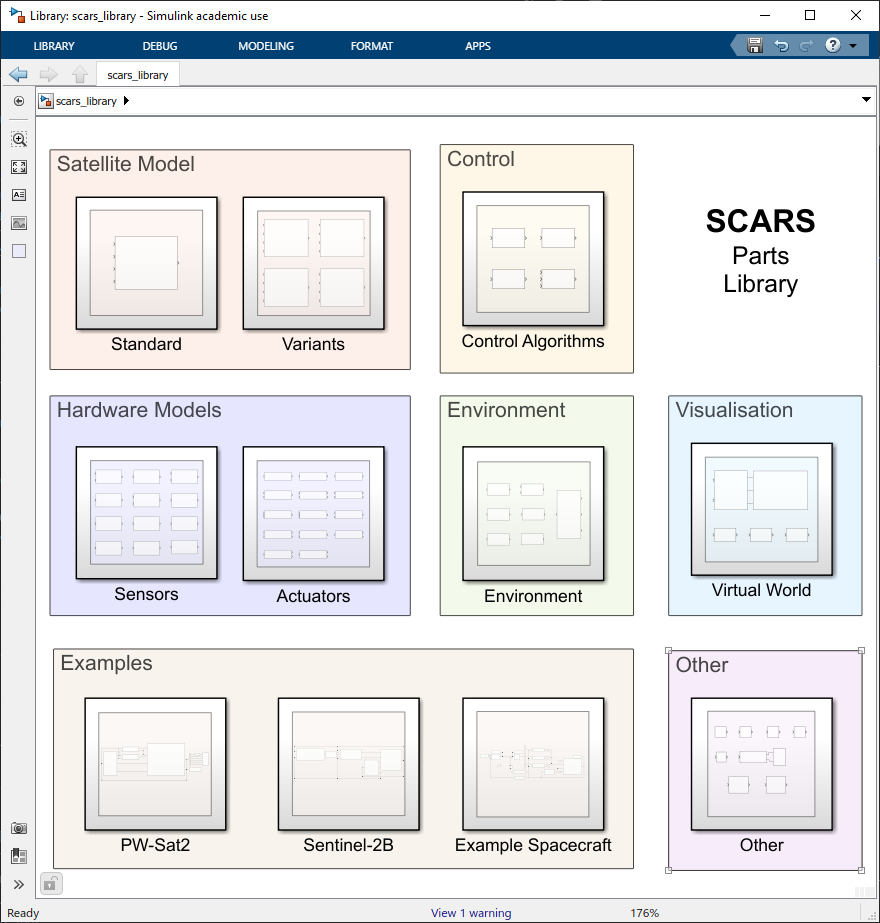
\includegraphics[width=1\textwidth]{2-toolbox/scars-library.png}
            \caption{SCARS Parts Library screenshot}
            \label{fig:scars-library}
        \end{figure}

    \subsubsection{Modular Simulation}
        \ac{scars} Modular Simulation is a ready-made simulink model available for setup using prepared scripts and \ac{scars} user interface. The model is a simulation of cube-shaped satellite, which can be set on specified orbit using various initialization methods, such as Keplerian elements in conjunction with Julian date time. (The initialization is further described in Chapter \ref{sec:documentation}). In the same manner, all actuators and sensors available in \ac{scars} library can be chosen. The Modular Simulation makes use of most available blocks, which can be commented out from the model, either by hand or using the user interface, to improve the speed of the simulation.

        \begin{figure}[H]
            \centering
            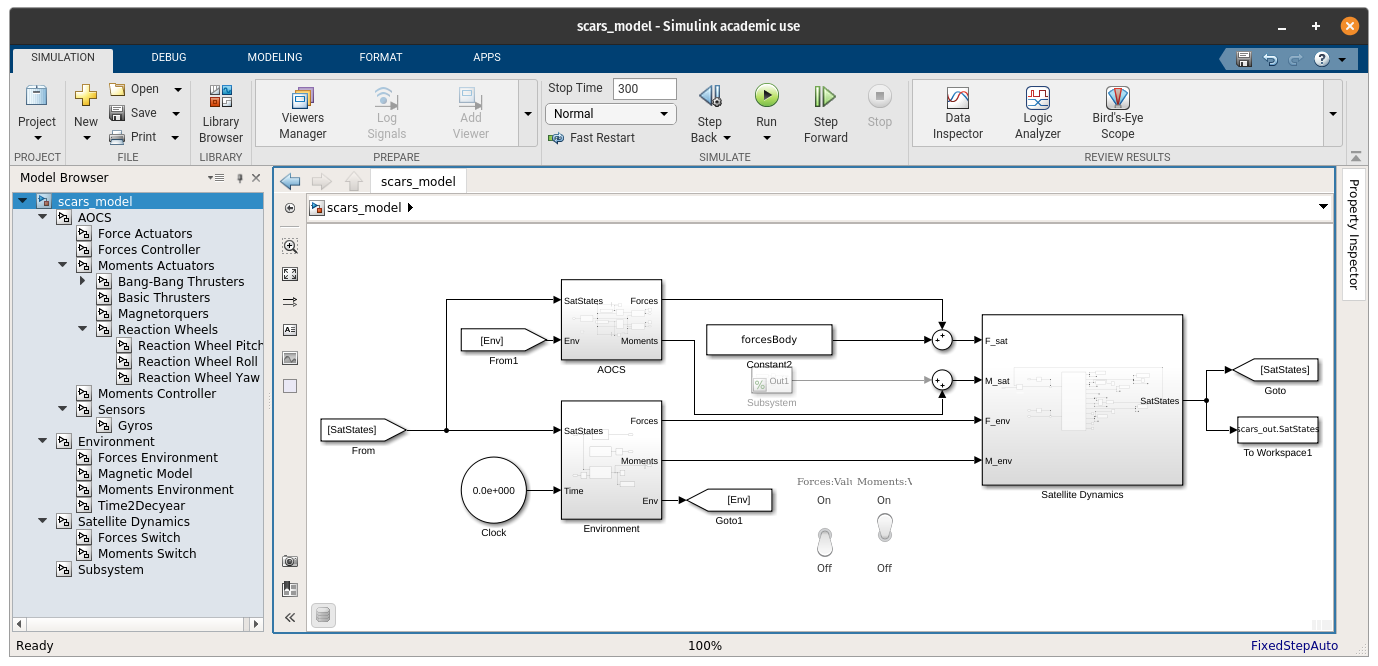
\includegraphics[width=1\textwidth]{2-toolbox/scars-model.png}
            \caption{SCARS Modular Simulation screenshot}
            \label{fig:scars-model}
        \end{figure}


    \subsubsection{Main Signal Buses}\label{sec:buses}
        To unify the signals transferred to blocks modelled in \ac{scars} Toolbox a pair of Simulink signal buses is proposed - \textbf{SatStates} bus, produced as the output of \textbf{Satellite Dynamics} block and \textbf{Env} bus, collected as an output of \textbf{Environment} block. Since the buses are unified, there is no need for unit or coordinate transformations between, for example, satellite model and sensor model. Following tables present descriptions of signals contained in designed buses. Reference frames mentioned here are explained in \autoref{sec:frames}. 
        
        % \dots \textit{pro Table below contains the description of signals contained in the}\dots 

        \begin{table}[H]
            \begin{tabularx}{\textwidth}{llXl}
            \textbf{Name} & \textbf{Unit} & \textbf{Description} & \textbf{Size} \\ \hline
            V\_ECEF & m/s & Velocity of the body in ECEF frame, in relation to ECEF reference frame & 1x3 \\
            X\_ECEF & m & Position of the body in ECEF reference frame & 1x3 \\
            lla & deg, deg, m & Body latitude, longitude and altitude in reference to Earth's Geographical coordinates & 1x3 \\
            Euler\_NED & rad & Body rotation angles in relation to NED reference frame &  \\
            DCM\_ECI2B & - & Direction Cosine Matrix describing rotation from ECI frame to body frame & 3x3 \\
            DCM\_NED2B & - &  Direction Cosine Matrix describing rotation from NED frame to body frame & 3x3  \\
            DCM\_ECEF2NED & - & Direction Cosine Matrix describing rotation from ECEF frame to NED frame & 3x3  \\
            DCM\_ECEF2B & - &  Direction Cosine Matrix describing rotation from ECEF frame to body frame & 3x3  \\
            V\_B & m/s & Body acceleration in relation to its inertial reference frame &  1x3 \\
            Omega\_NED & rad/s & Body rotation rate in reference to NED reference frame & 1x3  \\
            Omega\_B & rad/s & Body rotation rate in reference to its inertial reference frame  & 1x3 \\
            Euler\_B & rad & Body's rotation angles in relation to its initial position  & 1x3 \\
            dOmega\_B/dt & rad/$s^2$ & Derivative of body rotation rate in reference to its inertial reference frame & 1x3 \\
            A\_B & m/$s^2$ & Body acceleration in relation to its inertial reference frame & 1x3 \\ \hline
            \end{tabularx}
            \caption{\textbf{SatStates} bus signals description}
        \end{table}

        Since \textbf{SatStates} bus contains ideal values of satellite states, the models that use it do so for purpose of modelling mechanical relations between satellite's frame and its hardware components. For other applications, like creation of control loop, it is advised to use sensor models instead.

        
        \begin{table}[H]
            \begin{tabularx}{\textwidth}{llXl}
            \textbf{Name} & \textbf{Unit} & \textbf{Description} & \textbf{Size} \\ \hline
            Magnetic Field [nT] & $nT$ & Strength of the magnetic field on Earth's orbit, depending on altitude, position and time & 1x3 \\
            Environment Force [N]& $N$ & Force acting on a spacecraft - a sum of gravitational pull and atmospheric drag & 1x3 \\
            Sun's Position [km] & $km$ & Position of the Sun with reference to Earth, in ECEF frame & 1x3 \\
            Atmosphere Density [km/m3]& $kg/m^3$ & Density of atoms in partial atmosphere at body's altitude & 1 \\ \hline
            \end{tabularx}
            \caption{\textbf{Env} bus signals description}
        \end{table}

        \textbf{Env} signal bus contains information about parameters of the environment at spacecraft coordinates. ALthough the values are derived from used models, they should be treated as ideal values, therefore for applications where the measurement is used as algorithm input, for example in B-Dot controller described in \autoref{sec:bdot} it is suggested to use a sensor model between \textbf{Env} block and actuator or \ac{obc} model.  